\section{幾何表示與互動式繪圖}

\subsection{圖形的幾何表示}
\label{sec:geometry-representation}

不同工具取得圖形的方法不一樣，但完成繪圖後都會將 Line、Rectangle、Path 和 Polygon 都整理成頂點序列，另外記錄路徑是否封閉。
Ellipse 則先由外接矩形算出中心和半徑，再取樣成 64 個頂點。Point 只需要位置；Text 會保存基準位置、UTF-8 字串和文字樣式。

這樣做的好處是 Renderer 和 Select Tool 都可以使用同一份幾何資料，不需要知道頂點原本是用拖曳、連續移動還是多次點擊產生的。

\subsection{互動式 Draft}
\label{sec:draft}

使用者在拖曳 Line 或 Rectangle 時，圖形還沒正式完成，但畫面上仍要即時預覽。這種暫時圖形稱為 Draft。
滑鼠移動只會更新 Draft，Canvas 再把它畫在原本的 Scene 上面；等到使用者放開滑鼠或完成 Polygon，才把 Draft 轉成正式物件並加入 Document。

這個做法也讓 Undo 比較單純。一次拖曳雖然會收到很多 Motion event，最後只建立一筆 Command；
如果繪圖途中按 Undo，程式會先取消目前 Draft，而不是刪除上一個已完成物件。

\begin{figure}[htbp]
    \centering
    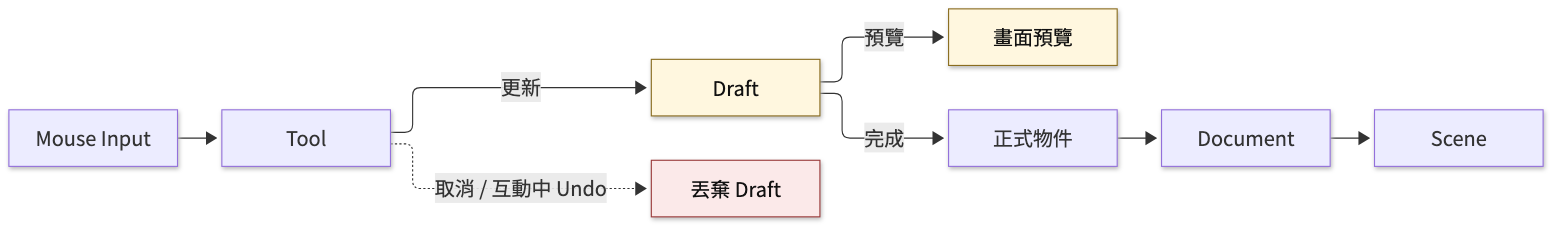
\includegraphics[width=.92\textwidth]{docs/figures/ch04_draft-flow.png}
    \caption{Draft 從滑鼠輸入、預覽到提交成正式物件的流程}
    \label{fig:draft-flow}
\end{figure}

\subsection{Pencil 路徑採樣}
\label{sec:pencil-sampling}

Pencil 需要一直收集滑鼠位置，但如果把每個 Motion event 都存下來，會產生很多幾乎重合的點。
設上一個採樣點為 $P_{i-1}$、目前位置為 $P$、線寬為 $w$，最小距離設為
\[
    d_{\min}=\max(0.2w,1\text{ px}).
\]
只有 $\norm{P-P_{i-1}}\ge d_{\min}$ 時才加入新點。除了減少資料量，這也能避免很短的線段讓後面的法向量和轉角計算變得不穩定。
